\chapter{电路设计与仿真}

本章对基于Cadence Virtuoso仿真软件和SMIC 0.18um BCD工艺设计的变换器芯片的各个关键电路进行分析和仿真,包括欠压锁定电路、内部供电电路、模式切换电路、退磁时间动态校准电路、峰值电流控制电路、精确谷底导通电路、谷值锁定电路、逻辑控制电路和各个保护电路等。最后对整体电路进行系统仿真,测试变换器芯片的基本功能,验证该电路设计的合理性和可靠性。

\section{欠压锁定电路}




\section{内部供电电路}

\subsection{带隙基准电路}

在变换器芯片工作过程中,其内部的各个模块都需要相应的偏置电压和偏置电流,为了维持这些偏置电压和偏置电流的精确和稳定性,不能用普通的与电源无关的基准电路产生全部的信号,因此需要设计带隙基准电路,提供受电源电压和温度变化影响很小的基准电压电流,使得变换器芯片适用于各种工况下。

带隙基准电路的实现原理是通过将一个正温度系数的电压和一个负温度系数的电压加权相加后,抵消掉其正负温度系数,得到不受温度变化影响的零温度系数的基准电压。实际电路中,负温度系数的电压利用双极型晶体管产生,其正向压降$V_{be}$带有负温度特性。通过半导体物理的基础知识可知,电压$V_{be}$的公式为:
\begin{equation}
    \label{eq:Vbe公式}
    V_{be} = V_T \cdot ln(\frac{I_c}{I_s})
\end{equation}
其中,$V_T$是热电压,公式为:
\begin{equation}
    \label{eq:VT公式}
    V_T=\frac{kT}{q}
\end{equation}
$I_c$是PN结的集电极电流,公式为:
\begin{equation}
    \label{eq:Ic公式}
    I_c=I_s \cdot exp(\frac{V_{be}}{V_T})
\end{equation}
$I_s$是PN结饱和电流,公式为:
\begin{equation}
    \label{eq:Is公式}
    I_s=bT^{4+m} exp\frac{-E_g}{kT}
\end{equation}
结合式\eqref{eq:Vbe公式}、\eqref{eq:Ic公式}和\eqref{eq:Is公式},通过正向压降$V_{be}$对温度求偏导,可计算得$V_{be}$的负温度系数公式:
\begin{equation}
    \label{eq:Vbe/T公式}
    \frac{\partial V_{be}}{\partial T} = \frac{ V_{be} - (4+m)V_T - E_g/q}{T}
\end{equation}

正温度系数的电压同样可以通过双极型晶体管来产生,不同电流密度的电流流经晶体管会产生不同的负温度系数,两者的差值电压$\varDelta V_{be}$带有正温度系数。实际电路中为了满足晶体管的匹配性,使用两个不同面积的双极型晶体管来产生不同电流密度的作用。令两个双极型晶体管的面积比为$1:N$,则流经单个晶体管的电流密度比N:1,可计算得晶体管压差$\varDelta V_{be}$的公式为:
\begin{equation}
    \label{eq:△Vbe公式}
    \varDelta V_{be} = V_T ln(\frac{I_c}{I_s}) - V_T ln(\frac{I_c}{nI_s}) = V_T \cdot ln(n)
\end{equation}
通过$\varDelta V_{be}$对温度求偏导可计算得正的温度系数公式:
\begin{equation}
    \label{eq:△Vbe/T公式}
    \frac{\partial \varDelta V_{be}}{\partial T} = \frac{k}{q}\cdot ln(n)
\end{equation}


由式\eqref{eq:Vbe/T公式}和\eqref{eq:△Vbe/T公式}计算可知,在常温T=300K的条件下,当$V_{be}\thickapprox $ 750 mV时,$V_{be}$的负温度系数约等于-1.5 mV/K,$\varDelta V_{be}$的正温度系数为0.087ln(n) mV/K。为了合理地产生零温度系数电压,防止双极型晶体管的面积太大,需对正负温度系数加权相加可得。

为了满足变换器芯片中的低压数字模块,



\subsection{高压LDO电路}

由辅助绕组产生的供电端电压对于片内的元器件而已电压过大且不够稳定,无法直接用于作为供电电压,需要设计用于产生稳定输出电压的低压线性稳压器电路,将供电端的高压转化为可为内部电路供电的电源电压输出。
\begin{figure}[htbp] 
    \centering
    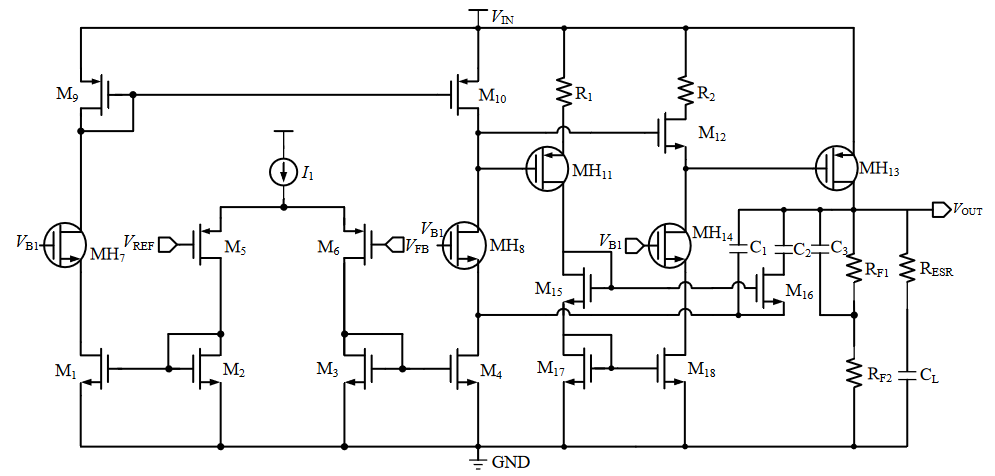
\includegraphics[width=0.6\linewidth]{figures/高压LDO.png}
    \caption{高压LDO电路图}
    \label{fig:高压LDO}
\end{figure}

本文设计的高压LDO电路如图~\ref{fig:高压LDO}所示,该电路


%\section{抖频振荡器}

\section{模式切换电路}

\section{退磁时间动态校准电路}

\section{峰值电流控制电路}

%\section{前沿消隐电路}

\section{精确谷底导通电路}

因为存在驱动器等电路的延时,为了实现精确的谷底导通功能,通过需要在$V_{HB}$谐振谷底到来之前产生低边功率管的导通逻辑信号,使得逻辑信号通过驱动器后,产生的实际控制低边功率管导通信号刚好处于$V_{HB}$信号谐振谷底的位置处,因此要求逻辑信号提前产生的时间等于驱动器等电路的延时时间。图~\ref{fig:精确谷底导通电路图1}是精确谷底导通信号的电路图。

LS和PLS分别是PWM控制电路产生的低边功率管控制信号和实际控制信号,通过逻辑控制电路得到LS和PLS信号的延时时间Pre\_Pulse。为了预判谷底信号,通过一个使用MOS管充当电阻的压控高通滤波器电路,产生$V_{ZCD}$对应的超前时间信号VHP\_ZCD,只需适当的调节VGS的大小即可控制VHP\_ZCD信号的超前时间大小。分别使用两个峰值检测电路来检测并得到两个信号的峰值脉冲信号,经过SR锁存器产生超前时间Deta\_Pulse。为了轻微的调节栅极电压信号VGS,使用了PLL电路中的鉴相鉴频器和电荷泵电路来控制Deta\_Pulse信号逐步逼近Pre\_Pulse信号,完成低边功率管的精确谷底导通功能。


\section{谷值锁定电路}

\section{逻辑控制电路}

\section{保护电路}

\section{系统整体仿真}

\section{小结}




